\documentclass[a4paper,11pt]{report}
\usepackage[utf8]{inputenc}
\usepackage{graphicx}
\usepackage{float}
\usepackage{caption}
\usepackage{subcaption}
\usepackage{amsmath}
\usepackage[table]{xcolor}
\usepackage{cite}
\usepackage{algorithm}
\usepackage{algpseudocode}

% Title Page
\title{Literature Review}
\author{Anna Ruth Rowan}


\begin{document}
\maketitle

\tableofcontents

\begin{abstract}
%AAAAAAAAAAAAAH
This project aims to explore different modelling methods for the morphogenesis of natural systems, focusing particularly on sea shells. It will compare different tactics such as aiming for visual similarity versus describing the underlying biological mechanics causing the patterns and perhaps also draw parallels between development at different levels of nature.
\end{abstract}

%\chapter{Introduction}

%\begin{itemize}
% \item Talk about how theres loads of different patterns in nature.
% \item spacio-temperal patterns - animal swarms as opposed to static ones like pattern in fur
% \item descriptive model vs explanitory model - reasons for modelling things
% \item good oppertunity for pictures...
%\end{itemize}

%Aim: To implement a few different models of pattern formation in natural systems. Staring with seashells and moving on to the development of more complex systems such as embryos.

\chapter{Literature Survey}

In this section I will describe the models that I intend to investigate over the coming project.
%\begin{itemize}
% \item ``I'm going to describe a few models''
% \item some references needed throughout
%\end{itemize}

\section{The Cellular Automaton Model}

A cellular automaton is an array of cells where each cell can change state depending on the states of its neighbours \cite{arsmith}. In its simplest form the cells make up a single row and can either be in an 'on' or 'off' state. For every iteration the rules are applied to all cells at once and a new row is generated. If every new row is printed beneath the old then the result is a two-dimensional array displaying space in one direction and time in the other. What makes CA an appropriate model for seashells is that the shells grow in a similar way; with a single line of growth along one end of the shell and with older rows still visible behind it.

For example, if we were to take eleven cells and the rule set:
\[000 = 0, 100 = 1, 010 = 1, 001 = 1, 110 = 1, 101 = 0, 011 = 0, 111 = 0 \]
Then set a random initial state:

\begin{center}
\begin{tabular}{|c|c|c|c|c|c|c|c|c|c|c|}
 \hline
 \cellcolor{black} & & \cellcolor{black} & \cellcolor{black} & & & & \cellcolor{black} & & \cellcolor{black} & \cellcolor{black} \\
 \hline
\end{tabular}
\end{center}

We calculate the next state by observing the neighbours of each cell and matching them with a rule from our set. The third cell in this case matches the rule ``$011$'' and so its next state will be $0$. There is an issue with the edges of the array, since they do not have two neighbours and so cannot match a rule. This can be overcome with several methods, such as to declare the space outside the array to be all 0's or all 1's. The most common method is to wrap the array into a ring so that the cells on the far left and far right become neighbours. Since most shells do not grown in rings, for the purpose of this exercise we will say that the missing neighbour of an edge cell is always 0. With this method we find that the next iteration look like this:

\begin{center}
\begin{tabular}{|c|c|c|c|c|c|c|c|c|c|c|}
 \hline
 \cellcolor{black} & & & \cellcolor{black} & \cellcolor{black} & & \cellcolor{black} & \cellcolor{black} & & & \cellcolor{black}\\
 \hline
 \end{tabular}
\end{center}

And the following:

\begin{center}
\begin{tabular}{|c|c|c|c|c|c|c|c|c|c|c|}
 \hline
 \cellcolor{black} & \cellcolor{black} & \cellcolor{black} & & \cellcolor{black} & & & \cellcolor{black} & \cellcolor{black} & & \cellcolor{black} \\
 \hline
\end{tabular}
\end{center}

By repeating the process and placing each row below the last we achieve this pattern:

\begin{center}
\begin{tabular}{|c|c|c|c|c|c|c|c|c|c|c|}
 \hline
 \cellcolor{black} & & \cellcolor{black} & \cellcolor{black} & & & & \cellcolor{black} & & \cellcolor{black} & \cellcolor{black} \\ \hline
 \cellcolor{black} & & & \cellcolor{black} & \cellcolor{black} & & \cellcolor{black} & \cellcolor{black} & & & \cellcolor{black}\\ \hline
 \cellcolor{black} & \cellcolor{black} & \cellcolor{black} & & \cellcolor{black} & & & \cellcolor{black} & \cellcolor{black} & & \cellcolor{black} \\ \hline
 & & \cellcolor{black} & & \cellcolor{black} & \cellcolor{black} & \cellcolor{black} & & \cellcolor{black} & & \cellcolor{black} \\ \hline
 & \cellcolor{black} & \cellcolor{black} & & & & \cellcolor{black} & & \cellcolor{black} & & \cellcolor{black} \\ \hline
 \cellcolor{black} & & \cellcolor{black} & \cellcolor{black} & & \cellcolor{black} & \cellcolor{black} & & \cellcolor{black} & & \cellcolor{black} \\ \hline
 \cellcolor{black} & & & \cellcolor{black} & & & \cellcolor{black} & & \cellcolor{black} & & \cellcolor{black} \\ \hline
 \cellcolor{black} & \cellcolor{black} & \cellcolor{black} & \cellcolor{black} & \cellcolor{black} & \cellcolor{black} & \cellcolor{black} & & \cellcolor{black} & & \cellcolor{black} \\ \hline
 & & & & & & \cellcolor{black} & & \cellcolor{black} & & \cellcolor{black} \\ \hline
 & & & & & \cellcolor{black} & \cellcolor{black} & & \cellcolor{black} & & \cellcolor{black} \\ \hline
 & & & & \cellcolor{black} & & \cellcolor{black} & & \cellcolor{black} & & \cellcolor{black} \\ \hline
\end{tabular}
\end{center}

It is worth noting here that the method used to deal with edge cases has a huge impact in a case like this with only eleven cells but would be less pronounced on a system like a sea shell with many thousands of cells. Still, depending on the rules, the effect of poorly matched edge rules could spread a long way.

\subsection{Uses}

Cellular automaton have been been used to explore various concepts, such as self-reproduction in automata, evolution and pattern recognition \cite{tessellation}, but what we are interested in is the occasional visual similarity between one-dimensional cellular automata and sea shells.

\begin{figure}[H]
 \centering
 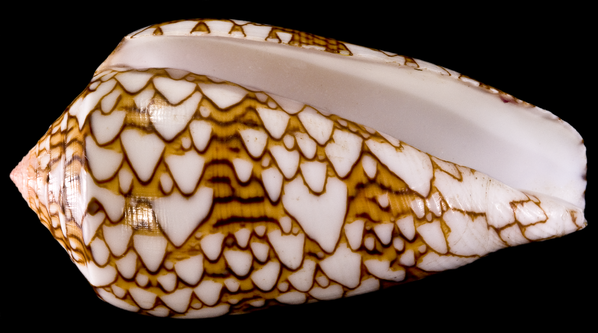
\includegraphics[scale=0.5]{images/conus_textile.png}
  \caption*{Source: $https\://commons.wikimedia.org/wiki/File\:C\%C3\%B4ne\_textileII.png$}
  \caption{Conus Textile}
\end{figure}
 
\begin{figure}[H]
 \centering
 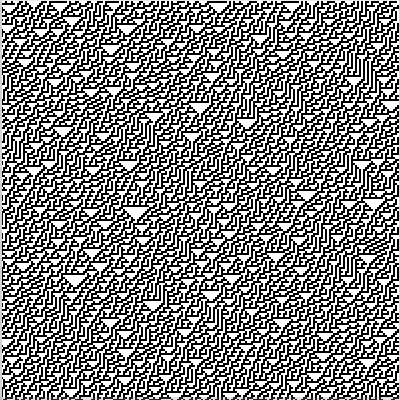
\includegraphics[scale=0.7]{images/ca_00011110.png}
 \caption*{Source: $https\://commons.wikimedia.org/wiki/Category\:Rule\_30\#/media/File\:Rule30\_sync.png$}
 \caption{A cellular automaton with the rule set 00011110}
\end{figure}

Here, figure 2.2 displays a similar random triangle pattern to the shell of Conus Textile in figure 2.1. With a few alterations - such as allowing a gradient of colours rather than a binary, or increasing the neighbourhood of a cell - it should be possible to create rough models of various sea shells. 

\section{The Activator-Inhibitor Model}

In the simplest activator-inhibitor model there are two interacting chemicals. The first acts as a catalyst for both chemicals and the second inhibits the growth of the first. Where $a$ is an activator, $b$ is an inhibitor and $c_a$ and $c_b$ are production constants, the system can be written like so:
\begin{equation}
 \begin{align}
 \frac{\partial a}{\partial t} &= c_a\frac{a}{b} \\
 \frac{\partial b}{\partial t} &= c_b a
\end{align}
\end{equation}

But this on it's own cannot be used to model pattern formation, for that we need interaction between neighbouring cells. The key to simulating unstable behaviours using this model is for the inhibitor to diffuse at a greater rate than the activator - this makes the relative concentrations of the chemicals at any one time far less predictable.
\begin{equation}
 \begin{align}
 \frac{\partial a}{\partial t} &= c_a\frac{a}{b} + d_a\frac{\partial ^2 a}{\partial x^2} \\
 \frac{\partial b}{\partial t} &= c_b a + d_b\frac{\partial ^2 b}{\partial x^2}
\end{align}
\end{equation}

Here, $d_a$ and $d_b$ represent the diffusion coefficients of the activator and inhibitor and $x$ the spatial coordinate. The reason that net increase from diffusion is related to the second derivative rather than the first is that if the gradient were linear for a particular cell, that would mean the flow of chemicals into the cell from one side would be equal to the flow of them leaving the cell to the other neighbour \cite{seashells}.

Following is a model described by Meinhardt \cite[p. 23]{seashells}:
\begin{equation}
 \begin{align}
  \frac{\partial a}{\partial t} &= s\bigg(\frac{a^2}{b} + p_a\bigg) - r_a a + d_a\frac{\partial ^2 a}{\partial x^2} \\
  \frac{\partial b}{\partial t} &= sa^2 - r_b b + d_b\frac{\partial^2 b}{\partial x^2} + p_b
 \end{align}
 \label{meinhardt_eq}
\end{equation}

This model takes a few more aspects into account, such as the rate of removal for both chemicals ($r_a$ and $r_b$) and the source density of the activator in a cell ($s$), which affects the rate of autocatalysis. There is also a base production level for both chemicals ($p_a$ and $p_b$) to allow a pattern to rekindle if it should die out.

%\section{The Algorithmic Beauty of Seashells}
%about application?
%\section{The Chemical Basis of Morphogenesis}
%about application?

\chapter{Requirements Analysis}
For the project to be complete, two models will need to be built: one being the adapted cellular automata and the other being the activator-inhibitor model. If there is ample time, it would good to also explore the effect of adding the flat models to three-dimensional shell shapes and to look into embryonic morphogenesis and the parallels between the different systems.
%\begin{itemize}
% \item what needs to be done to achieve the end/aim
% \item implement the two models
% \item both need visual outputs - render onto seashell shape
% \item method of user interaction
% \item explore the variables involved in both models - diffusion rates and such. How are they chosen?
%\end{itemize}

\section{General Requirements}
Both models will require a visual output displaying an array of coloured cells and preferably a form with which a user could easily alter the parameters of the model. There should also be the option of choosing a few preset configurations which model natural shell patterns.

%\begin{itemize}
% \item talk about common parameters and specific parameters for different shells and then for the different models
%\end{itemize}

\section{Modelling Seashells in CA}
In the case of the cellular model, the user should be able to alter which rule set the model is running - this is the minimum necessary functionality, but there are additional features that could be of use, such as increasing the neighbourhood of a cell either just in the spacial dimension or in both space and time. Doing this however would mean that the rule set - which is usually a list of outcomes for every possible configuration of the neighbourhood - would grow very large very quickly and become tedious to handle. One workaround would be use the method in Conway's Game of Life \cite{gameoflife} where the only the total value of the neighbourhood is considered, but this might 


\section{Modelling Seashells in I-H}
This will be the larger and more complex of the two models and so there are many more variables to play with. First and foremost are the values mentioned in the model equations \ref{meinhardt_eq}: so the base production values for the activator and inhibitor, the diffusion rates, the removal rates and the source density coefficient. Apart from this it may be interesting to compare different I-H model variations \cite[47-48]{turingmorph} and introduce the possibility of adding a trauma event  at random points, such as a shell fracture, or a temporary disappearance of the activator which might model a shortage or change in the diet of the creature. Related to this there may be annual cycles of plenty and shortage related to the seasons or the migration and food availability.

\section{Evaluating the Models}
Evaluating the models will be one of the more difficult parts of the project. The simplest would be to manually visually compare the output of the models with images of the target shell, but this is slow and laborious. Another option is to compare my model with existing models that are considered good by peers and use a pattern-recognition system to judge similarity, but this does not allow for the new model being possibly better in some respects to the older. I will need to put some more thought into this problem.

\chapter{Progress}

\section{The CA Generator}
I have created a simple cellular automaton generator in Python which takes the rule numbers as an input. It currently deals with edge cases using the standard method of wrapping the array into a cylinder which is convenient for testing that the model works, but this is incorrect for modelling shells. I will have to try a few different methods to find the optimal edge rules.

%\begin{itemize}
% \item Algorithm
% \item outputs
%\end{itemize}


%\chapter{Conclusions and Project Plan}

%\begin{itemize}
% \item Write an Activator-Inhibitor model in Python
% \item Use this to model sea shell patterns
% \item Add to the CA model, model the same sea shells using this
% \item Compare and contrast - relate to the biology
% \item A-H models multiple chemical interaction, CA only one.
% \item How these models relate to pattern formation in embryos
%\end{itemize}

\bibliography{literature_review}{}
\bibliographystyle{plain}

%\listoffigures

\end{document}          

% c.elegans
% look at the self-made tapestry phillip ball - talks about modelling patterns. There's an electronic version on uni lib
% have a look at editorials for writing style thoughts.